%latex.default(figure1)%
\documentclass{article}
\usepackage[pdftex]{graphicx}
\begin{document}
\begin{figure}
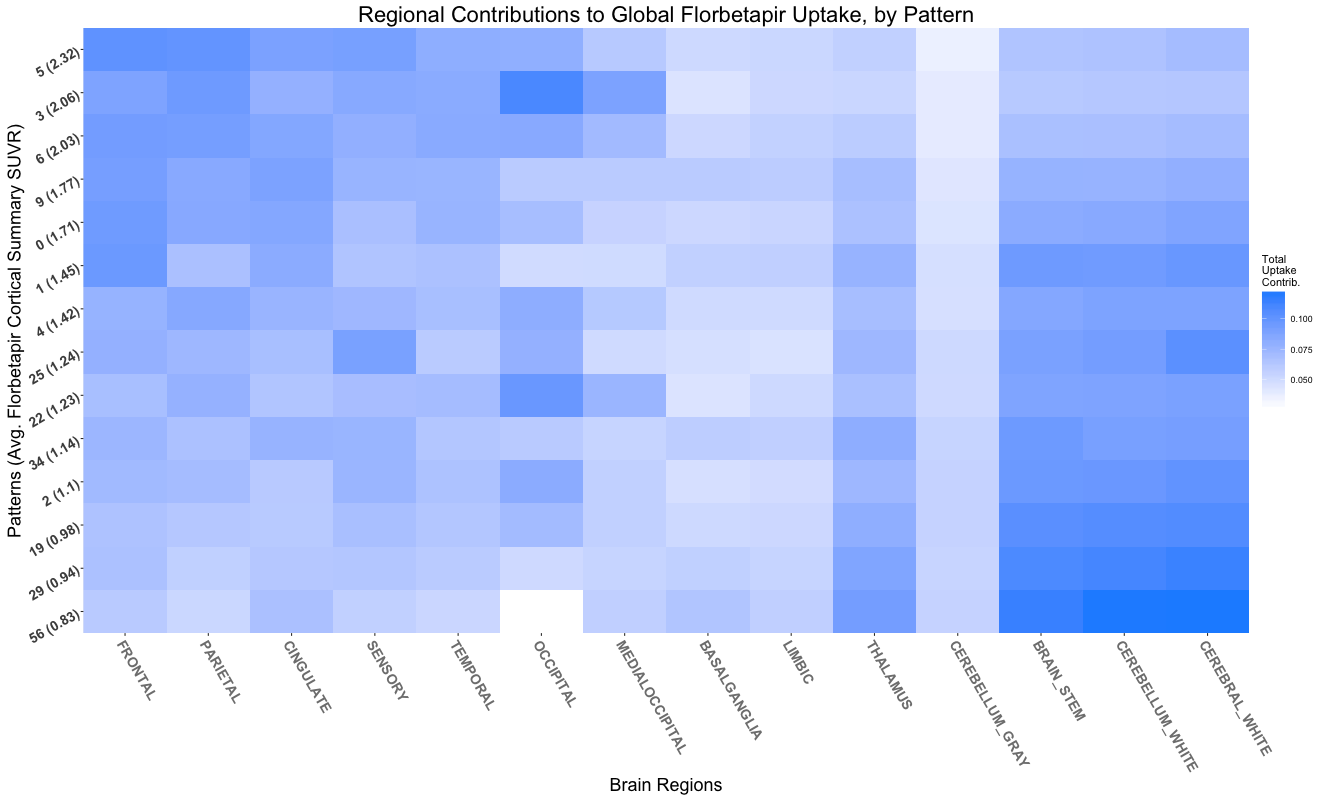
\includegraphics[width=125mm]{/usr/local/jagust/lobal_contributions.png}
\caption{By the perspective of total uptake contribution per region, i.e. regional SUVR divided by summed SUVR across all brain regions, we see that low-SUVR patterns exhibit dominant uptake in the cerebellum, brainstem, thalamus, and cerebral white matter regions, while uptake in high-SUVR patterns is dominated by the frontal, parietal, temporal, and cingulate cortices.}
\end{figure}

\begin{figure}
\includegraphics[width=125mm]{/usr/local/jagust/fitplot_sigregions.png}
\caption{On top of predicted annual change by other factors (represented by fit curve, factors include baseline cortical summary SUVR, age, education, and Apoe4 status), pattern groups 0,1, and 22 predict relative increases of between 0.01 and 0.02 SUVR/year while pattern group 25 correlates with an additional decrease of 0.02 SUVR/year.}
\end{figure}


\end{document}